%&"../virtual"

\begin{document}
    \title{虚拟机网络性能测试}
    \maketitle
    \section*{要求}
    Virtualized and bare metal network performance test.
    \begin{itemize}
        \item Download QEMU 5.2.0 from \href{https://www.qemu.org/download/}{https://www.qemu.org/download/} and compile.
        \item Create 2 VMs with TAP mode network (e1000 and virtio-net) by QEMU.
        \item Connect to your VM through VNC viewer or SSH.
        \item Compare the network performance (e1000 and virtio-net) of your host machine and VMs.
    \end{itemize}
    \section{连接交大云服务器}
    下面将使用 jCloud 虚拟机来完成实验。根据交大云关于 Linux 创建云主机的文档\cite{jcloudlinux},创建 Ubuntu 18.04 虚拟主机。并通过创建浮动 IP 的方式,创建一个可以用于本地访问的外网IP 地址。在安全组设置里放行 22 端口以启用 ssh 连接。

    \begin{figure}[H]
        \centering
        
\includegraphics[width=\linewidth]{jcloudhost}
        \caption{交大云主机}\label{fig:jcloudhost}
    \end{figure}

    使用 ssh 连接远程服务器\cite{jcloudssh},配置本地的 Windows Terminal\cite{winssh},以直接通过 ssh 连接服务器,见图 \ref{fig:jcloudssh}。通过 FileZilla 以方便地向服务器传输文件,见图 \ref{fig:filezilla}。

    \begin{figure}[H]
        \centering
        \begin{minipage}{0.48\textwidth}
            \centering
            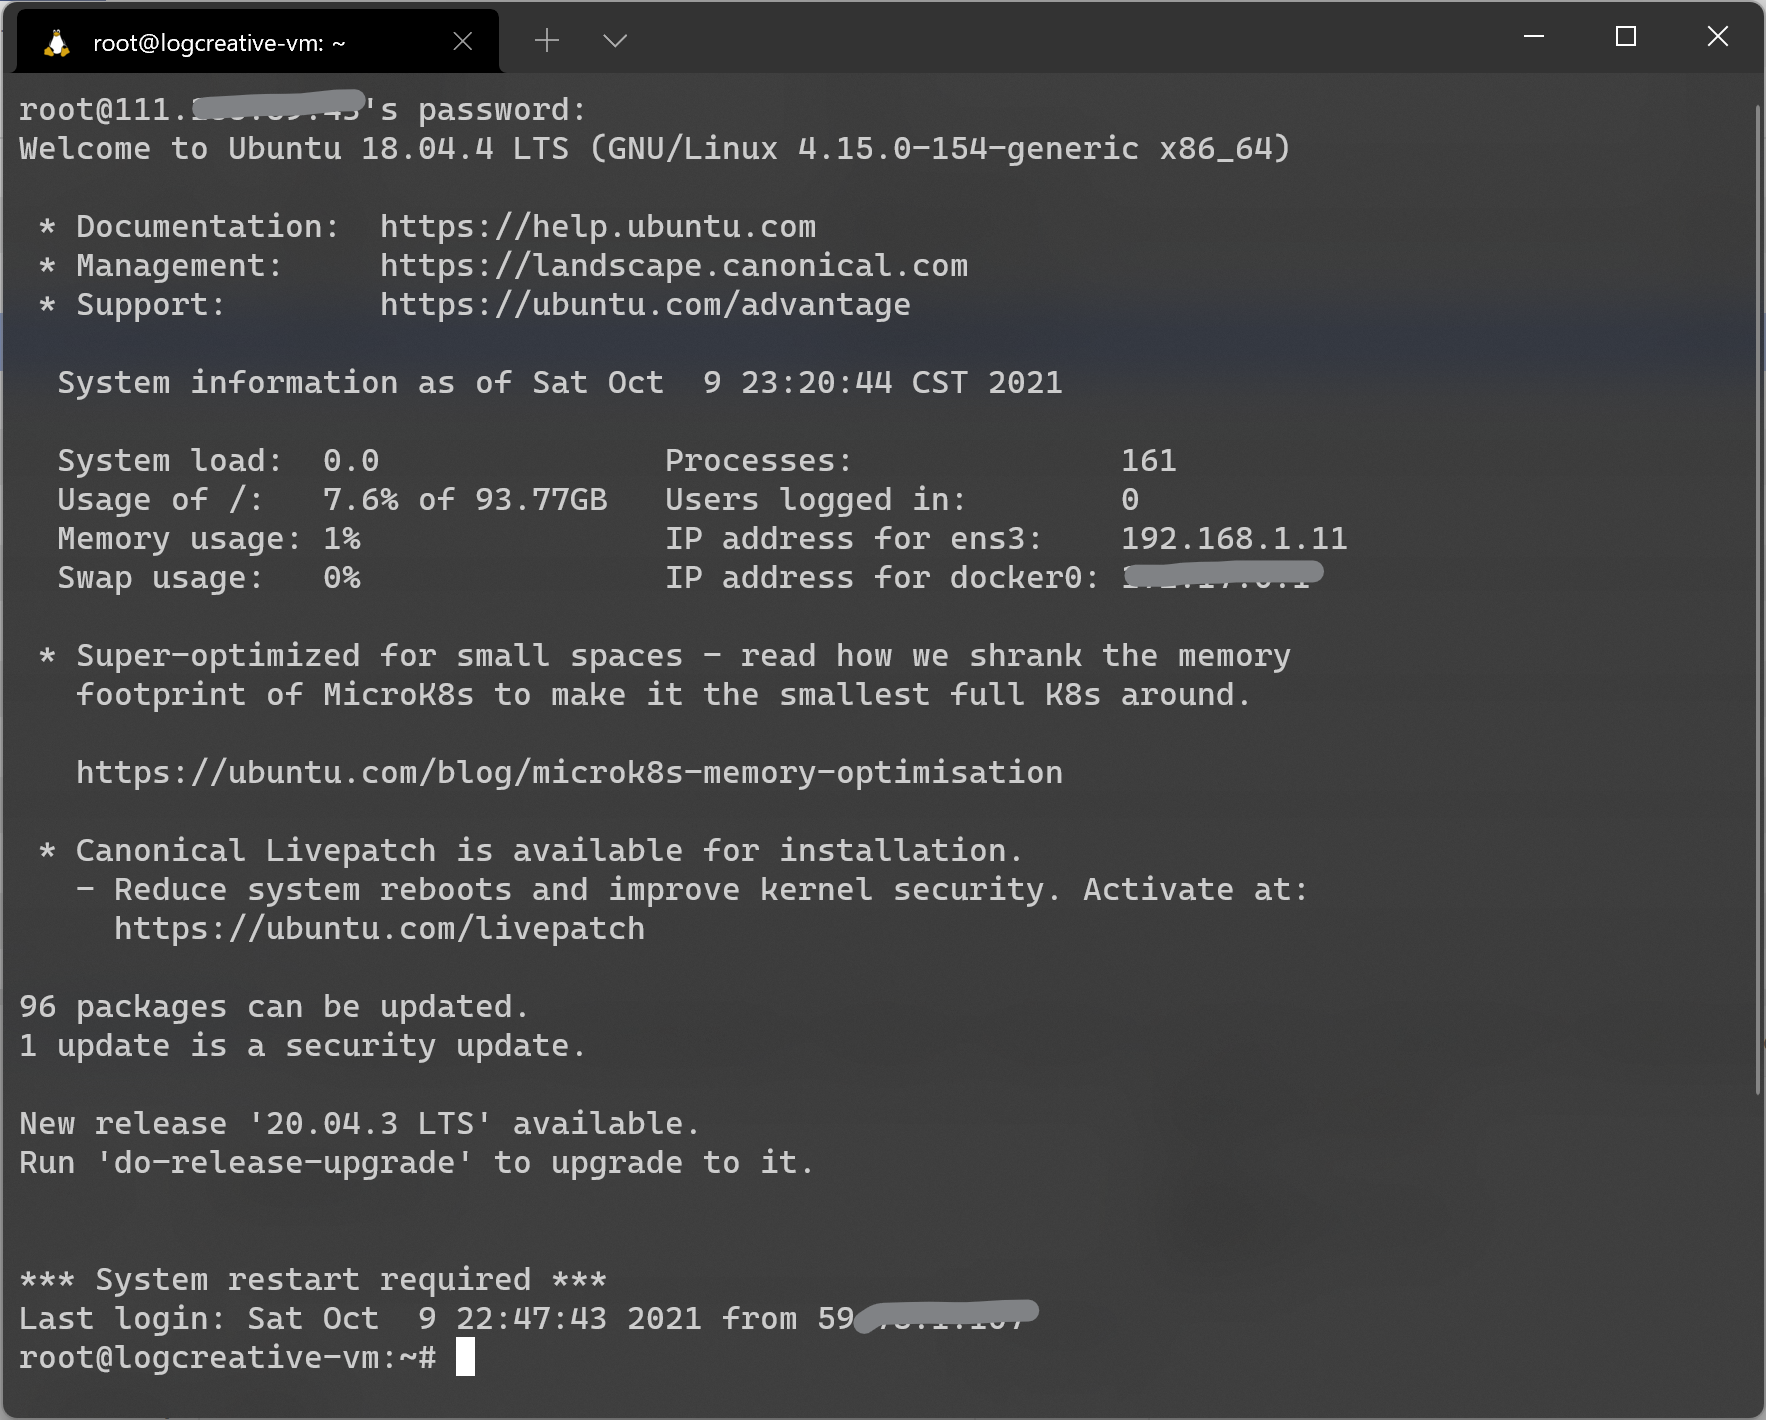
\includegraphics[width=\linewidth]{jcloudssh}
            \caption{通过 Windows Terminal 连接服务器}\label{fig:jcloudssh}
        \end{minipage}
        \begin{minipage}{0.48\textwidth}
            \centering
            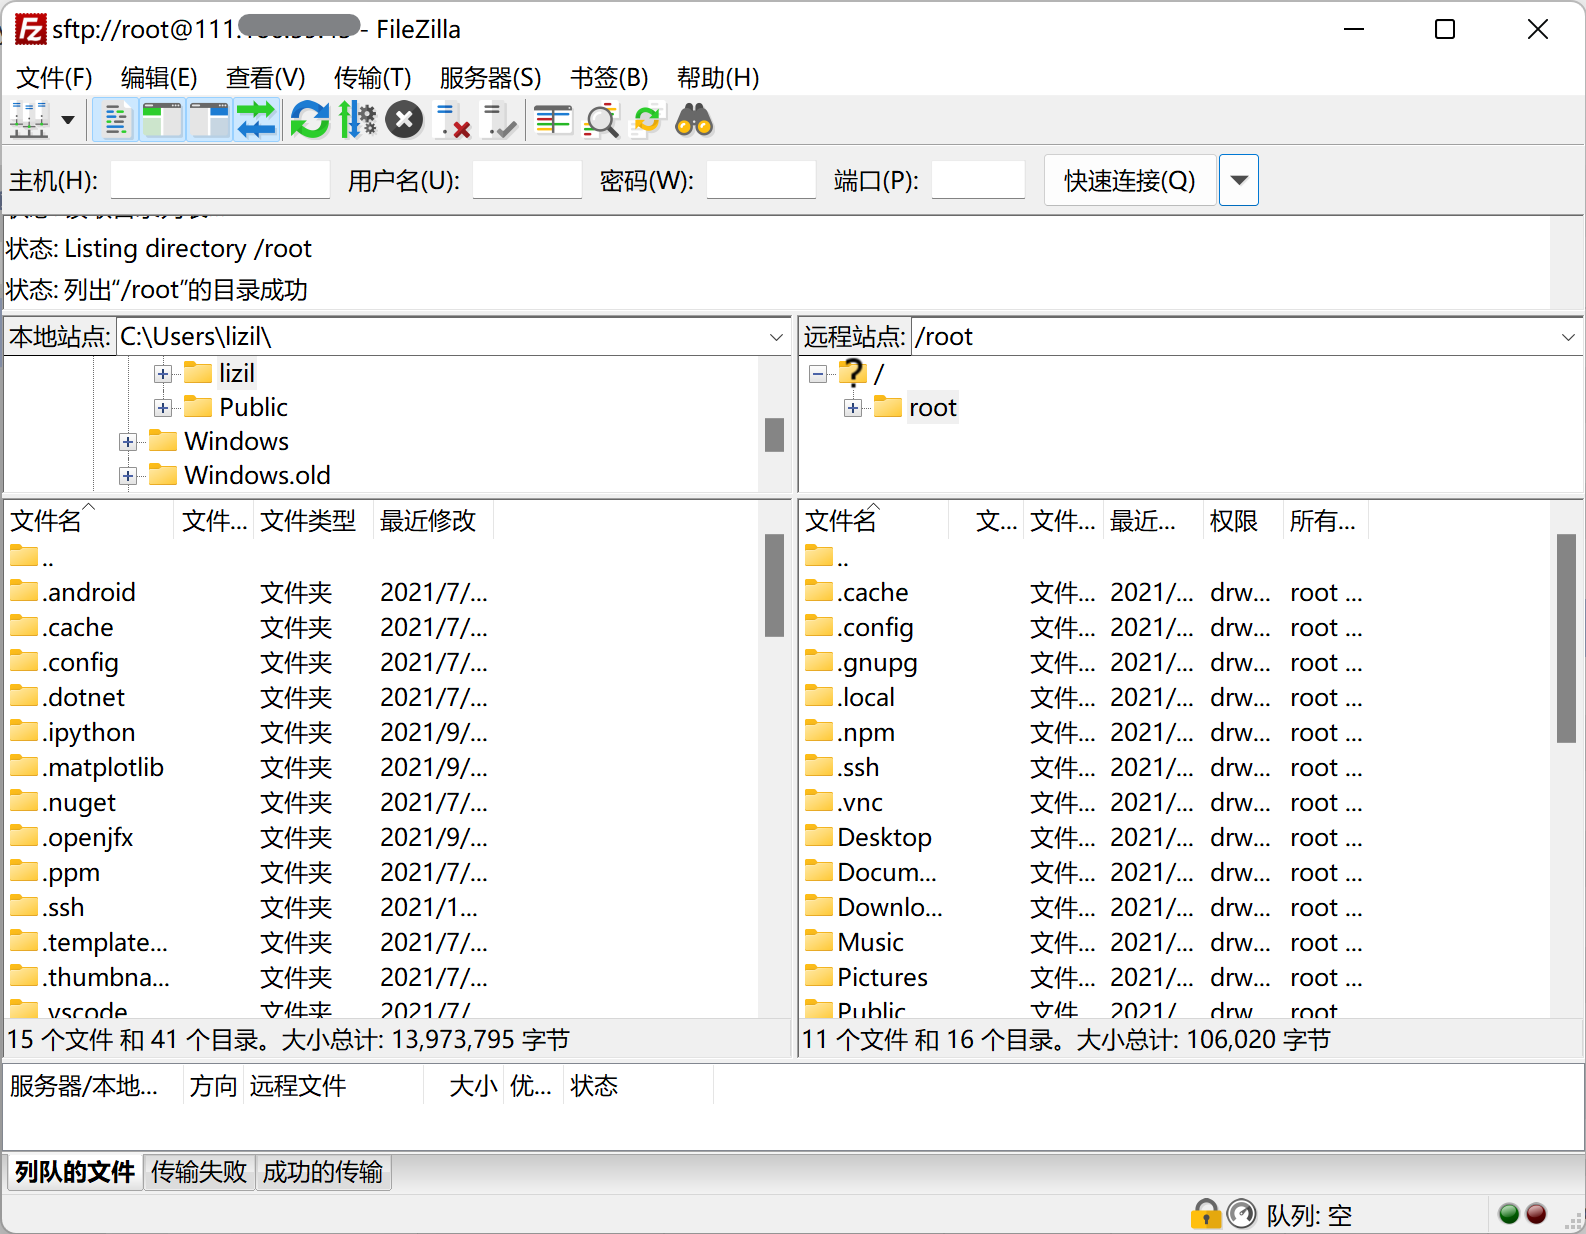
\includegraphics[width=\linewidth]{filezilla}
            \caption{使用 FileZilla 传输文件}\label{fig:filezilla}
        \end{minipage}
    \end{figure}

    % 放弃 VNC %%%%%%%
    % 通过下面的脚本在服务器上安装 VNC Server(顺带安装了 VNC Connect),并配置之\cite{vncconnect}。如图 \ref{fig:openport} 所示,在安全组设置里放行 5901 端口以启用 VNC 连接。

    % % su logcreative 切换用户
    % % 还需要设置用户组

    % \code[language=bash]{vnc.sh}

    % \begin{figure}[H]
    %     \centering
    %     \begin{minipage}{0.5\textwidth}
    %         \centering
    %         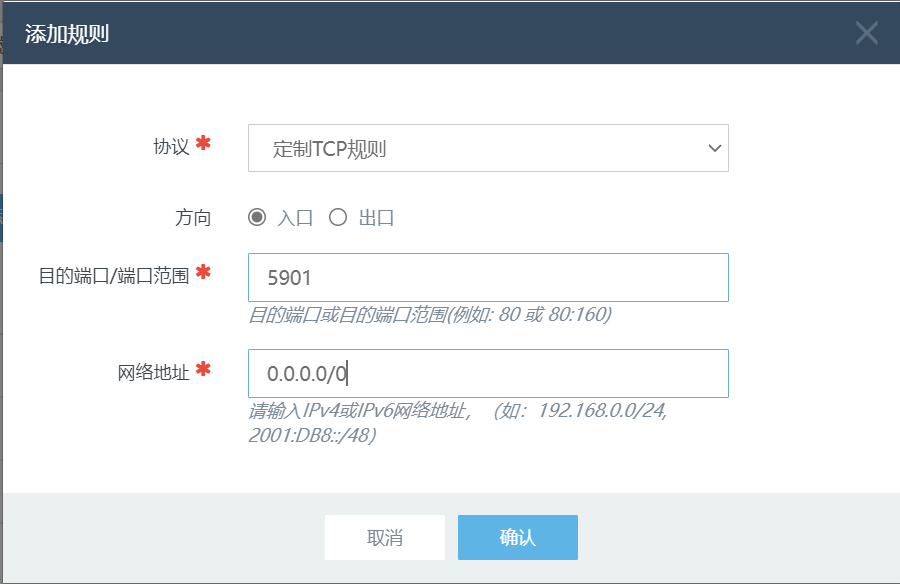
\includegraphics[width=\linewidth]{openport}
    %         \caption{放行 5901 端口}\label{fig:openport}
    %     \end{minipage}
    % \end{figure}

    \section{编译 QEMU}
    采用 QEMU 5.2.0 (Dec 8th 2020)。
    % 为了方便后续的版本对比,根据说明文档\cite{readme}直接克隆存储库。
    根据官方的 wiki 说明\cite{installwiki},需要安装一些额外包。通过下面的脚本进行下载、编译:
    \code[language=bash]{INSTALL.sh}
    其中 \verb"libvte-2.90-dev" 包已经被废弃。编译如图 \ref{fig:compile} 所示成功,安装如图 \ref{fig:install} 所示成功。
    \begin{figure}[h]
        \centering
        \begin{minipage}{0.48\textwidth}
            \centering
            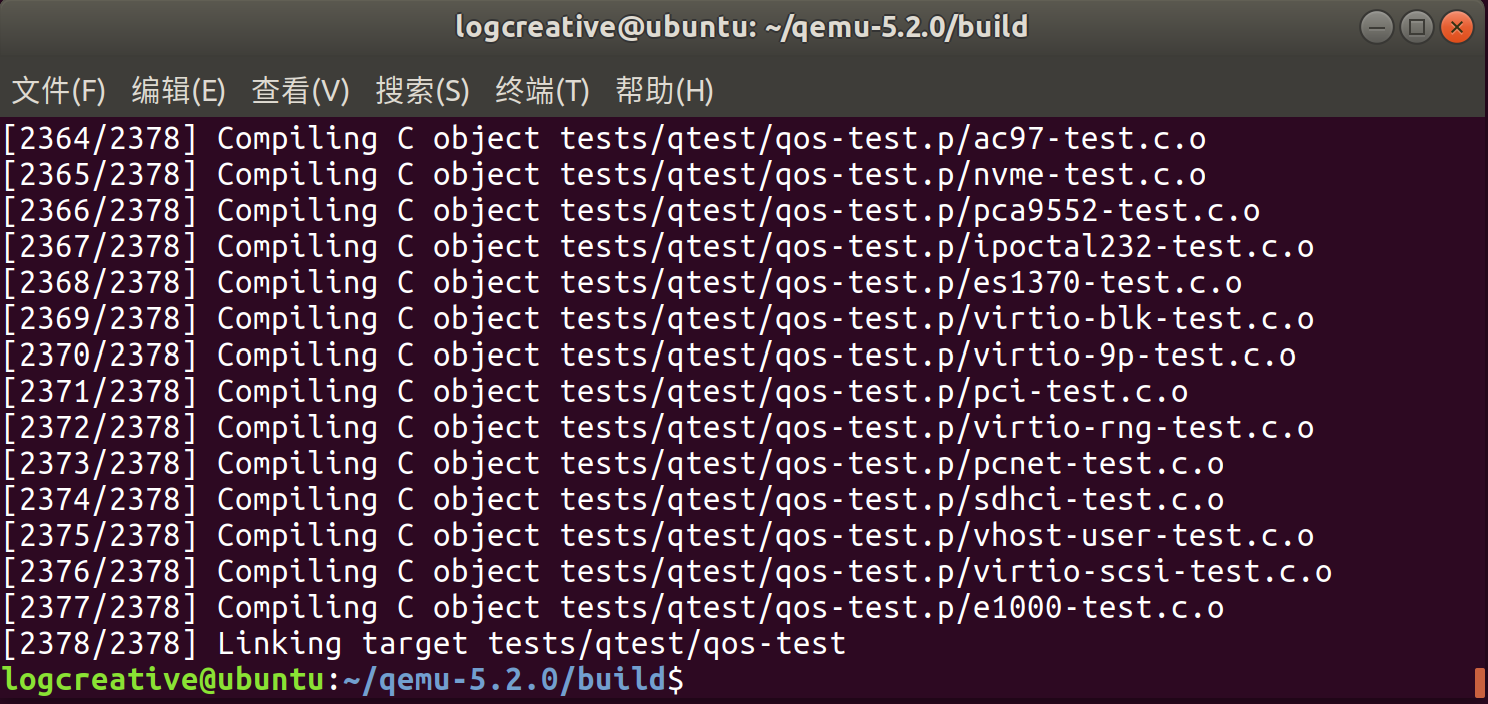
\includegraphics[height=3.1cm]{compile}
            \caption{QEMU 编译}\label{fig:compile}
        \end{minipage}
        \begin{minipage}{0.48\textwidth}
            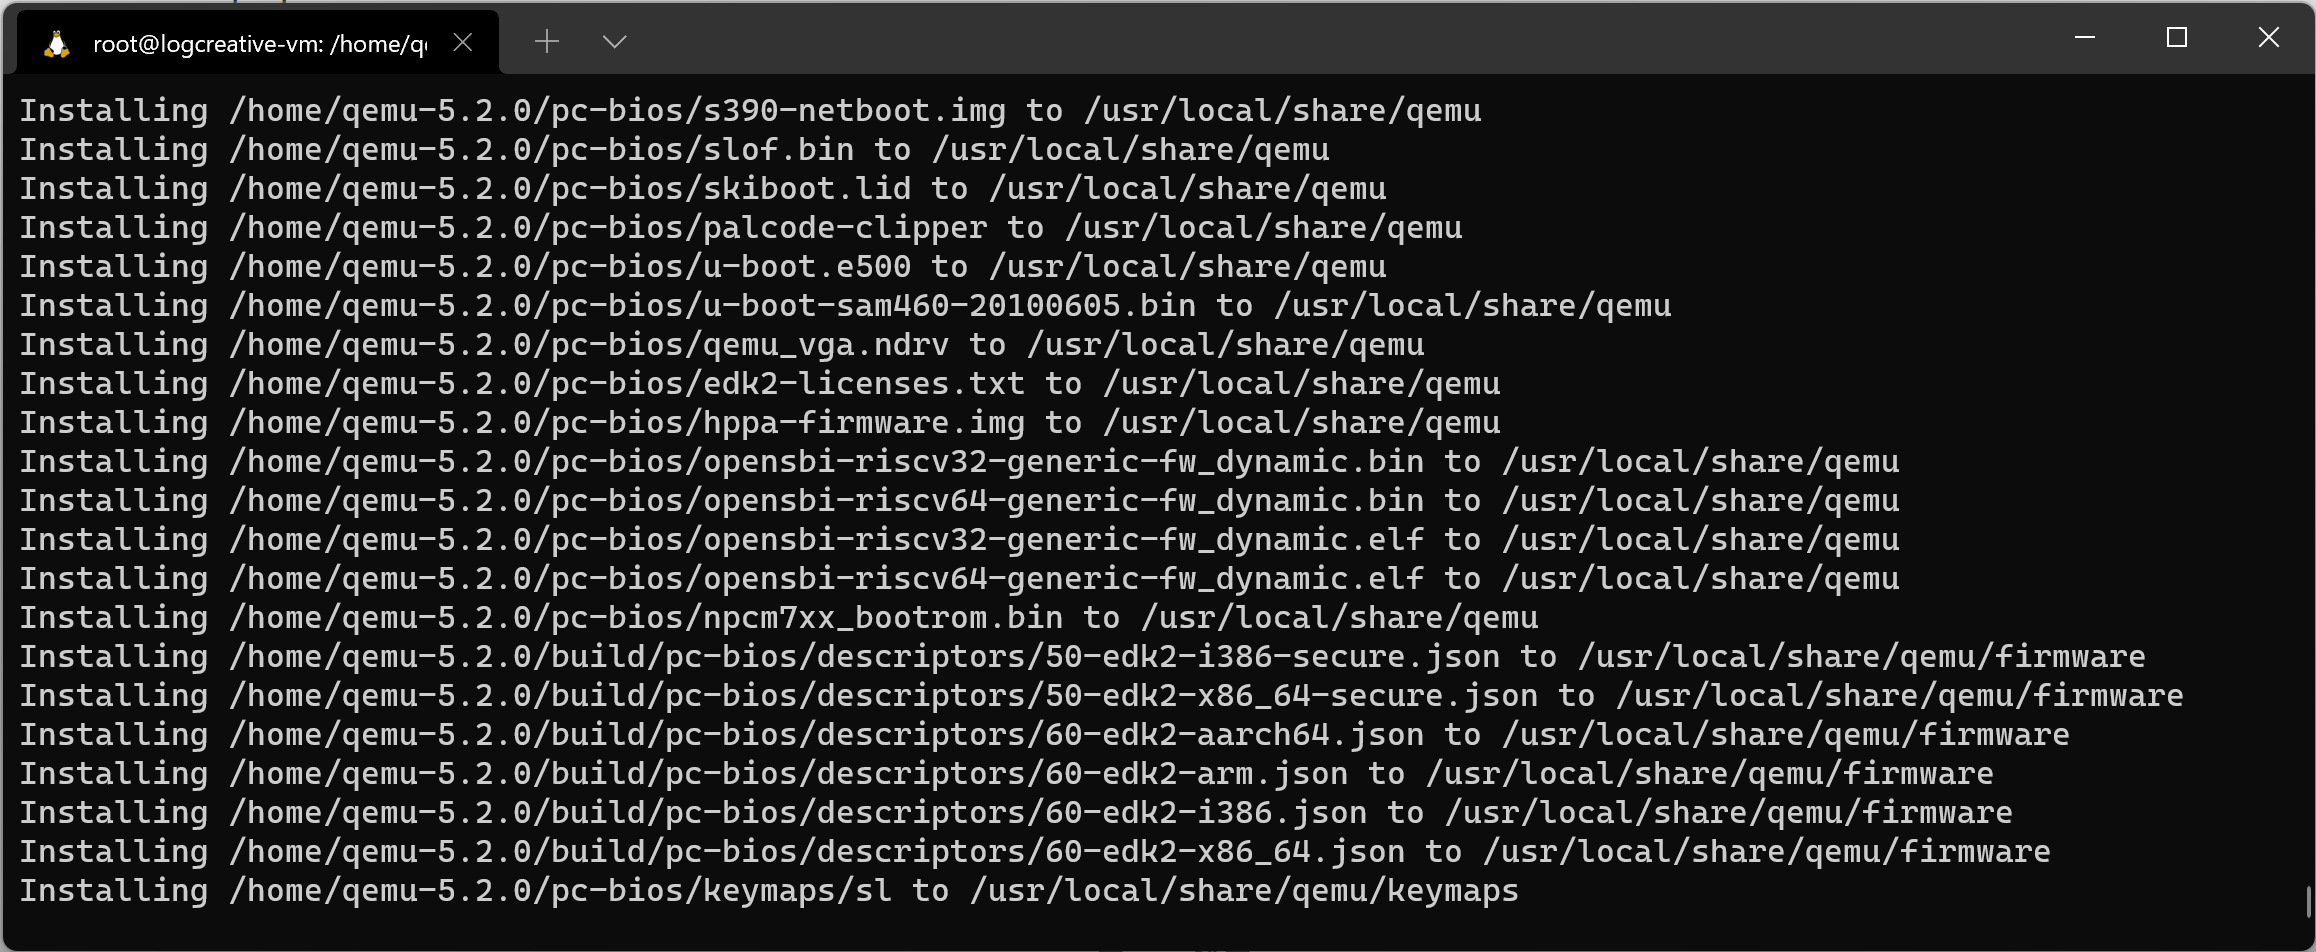
\includegraphics[width=\linewidth]{install}
            \caption{QEMU 安装}\label{fig:install}
        \end{minipage}
    \end{figure}

    % 对于 git clone,需要考虑更多的问题,这里略过。
    % 实际上,这里使用了 git submodule add https://git.sjtu.edu.cn/sjtug/qemu.git
    % 来插入子模块,并且需要使用
    % git submodule update --init --recursive
    % 来刷新内部的子模块
    % 如果出现问题,需要先使用
    % git submodule deinit --all -f
    % 来解除初始化

    \section{创建虚拟机}

    由于云主机不支持硬件虚拟化技术。

    \bibliography{ref}
\end{document}